%\documentclass[12pt,graphicx,caption,rotating]{article}
\documentclass[12pt,a4paper,spanish,twoside]{article}
\usepackage[paper=a4paper,top=3cm,bottom=3cm,left=3cm,right=3cm]{geometry}


% Separación de los párrafos
\setlength{\parskip}{0.6cm}

\usepackage[utf8]{inputenc}
\usepackage[spanish]{babel}
\usepackage [T1]{fontenc}
\usepackage{wrapfig} % Para permitir un gráfico al lado de texto
\usepackage{url}
\usepackage{epsfig}

\usepackage{titlesec}

% Graficos en párrafos
\usepackage{picins}

% Tablas muy largas que ocupan más de una página (se parten)
\usepackage{longtable}

%Paquete para subrayado, tachado, etc
\usepackage{ulem}
\normalem

% Incluir paragraph
\setcounter{secnumdepth}{4}
\setcounter{tocdepth}{4}
\makeatletter
\renewcommand\paragraph{\@startsection{paragraph}{4}{\z@}%
                                     {-3.25ex\@plus -1ex \@minus -.2ex}%
                                     {1.5ex \@plus .2ex}%
                                     {\normalfont\normalsize\bfseries}}
\makeatother

% Cambiar margenes en medio del texto
%\usepackage{chngpage}
%\usepackage{anysize}

\usepackage{listings}
\usepackage{color}
\definecolor{listinggray}{gray}{0.9}
\lstset{language=Matlab}
\lstset{keywordstyle=\color{red}\bfseries\underbar}

% Control de apendices
%\usepackage{appendix}
%\usepackage[toc,page]{appendix}

% Usar encabezados y pie de página
\usepackage{fancyhdr}

% Para cambiar el tipo de letra del ambiente verbatim
\usepackage{fancyvrb}
%\fvset{fontshape=it, fontfamily=courier}
%\DefineShortVerb{\|}

% Incluir los índices y la bibliografia en el índice general
%\usepackage{tocbibind}
\usepackage[nottoc]{tocbibind} % Saca todos los índices y la bibliografia al índice general y no pone este

\makeatother
\usepackage[pageref]{backref}
\renewcommand{\backreftwosep}{ y~}
\renewcommand{\backreflastsep}{ y~}

% Copy&paste de la doc de backref
% Mejorado con código "by Jelby"
\renewcommand*{\backref}[1]{}   % No usamos este hook, sino backrefalt
%
\renewcommand{\backrefalt}[4]{%
\ifcase #1 %
{\unskip\nobreak\hfil\penalty50\null\hfil%
\mbox{\nobreakspace\small[\textsl{No citado: usado como
referencia}]}%
\parfillskip=0pt\finalhyphendemerits=0\par}
\or
{\unskip\nobreak\hfil\penalty50\null\hfil%
\mbox{\nobreakspace\small[\textsl{Citado en
p\'ag.\nobreakspace#2.}]}%
\parfillskip=0pt\finalhyphendemerits=0\par}
\else
{\unskip\nobreak\hfil\penalty50\null\hfil%
\mbox{\nobreakspace\small[\textsl{Citado en
p\'ags.\nobreakspace#2.}]}%
\parfillskip=0pt\finalhyphendemerits=0\par}
\fi
}

% Para cambiar el espaciado en el índice
\usepackage{setspace}
\setlength\headheight{14.6pt}
\begin{document}
% Cambiar el nombre de cuadros a tablas (ponerlo en esta ubicación)
\renewcommand{\tablename}{Tabla}
\renewcommand{\listtablename}{Indice de tablas}


\begin{titlepage}

\vspace{4.3cm}

\begin{flushright}
{\large \bf Informe Técnico - Technical Report}\\
{\large \bf DPTOIA-IT-BORRADOR}\\
{\large \bf septiembre, 2006}
\end{flushright}

\begin{center}
\vspace{5.2cm}
{\Large \bf Plantilla Latex para Informes Técnicos}\\

\vspace{2cm}
{\bf Creada por Jesús Fernández Hernández}\\
{\bf Revisada por José Luis Alonso Berrocal}\\
{\bf Revisada por Roberto Therón Sánchez}\\
{\bf Autor 4}\\
\end{center}

%\vspace{5.9cm}
\vspace{1.9cm}
\begin{figure}[h!]
\begin{center}
\footnotesize

\includegraphics[width=5.94cm]{figures/usal_en_ver.jpg} % Filename.eps

\includegraphics[width=4.88cm]{figures/LogoDIA.jpg} % Filename.eps
\end{center}
\end{figure}

\vspace{1.5cm}
\begin{center}
{\bf Departamento de Informática y Automática}\\
{\bf Universidad de Salamanca}
\end{center}
\end{titlepage}

% Quitamos la numerac9i�n en esta p�gina
\thispagestyle{empty}
\vspace{4.9cm}
\begin{flushleft}
Revisado por:\\
\hspace{1cm}{Dr. - Pendiente de Asignar -}\\
\hspace{1cm}{Dr. - Pendiente de Asignar -}

\vspace{1cm}
%\vspace{1.3cm}
Aprobado en el Consejo de Departamento de <<fecha>>

\vspace{1cm}
%\vspace{2cm}
Información de los Autores:\\[0.5cm]

\hspace{1cm}{\footnotesize Autor 1}\\
\hspace{1.5cm}{\footnotesize 1ª Línea Autor1 }\\
\hspace{1.5cm}{\footnotesize 2ª Línea Autor1}\\
\hspace{1.5cm}{\footnotesize 3ª Línea Autor1}\\
\hspace{1.5cm}{\footnotesize Correo Autor1}\\[0.5cm]

\hspace{1cm}{\footnotesize Autor 2}\\
\hspace{1.5cm}{\footnotesize 1ª LíneaAutor2 }\\
\hspace{1.5cm}{\footnotesize 2ª Línea Autor2}\\
\hspace{1.5cm}{\footnotesize 3ª Línea Autor2}\\
\hspace{1.5cm}{\footnotesize Correo Autor2}\\[0.5cm]

\hspace{1cm}{\footnotesize Autor 3}\\
\hspace{1.5cm}{\footnotesize 1ª Línea Autor3 }\\
\hspace{1.5cm}{\footnotesize 2ª Línea Autor3}\\
\hspace{1.5cm}{\footnotesize 3ª Línea Autor3}\\
\hspace{1.5cm}{\footnotesize Correo Autor3}\\[0.5cm]

\hspace{1cm}{\footnotesize Autor 4}\\
\hspace{1.5cm}{\footnotesize 1ª Línea Autor4 }\\
\hspace{1.5cm}{\footnotesize 2ª Línea Autor4}\\
\hspace{1.5cm}{\footnotesize 3ª Línea Autor4}\\
\hspace{1.5cm}{\footnotesize Correo Autor4}\\[0.5cm]

\vspace{2.7cm}
%Este trabajo ha sido parcialmente financiado por

%\vspace{2.6cm}
\vfill
Este documento puede ser libremente distribuido.\\
(c) 2006 Departamento de Informática y Automática - Universidad de Salamanca.
\end{flushleft}

\newpage
% Ponemos numeraci�n romana y desde 1
%\pagenumbering{roman}
\renewcommand{\thepage}{\roman{page}} 
\setcounter{page}{1} 
\pagestyle{fancy}
\fancyhf{}
\fancyfoot[LE,RO]{\textbf{\thepage}}
\fancyfoot[LO,RE]{\textbf{DPTOIA-IT-BORRADOR}}
\renewcommand{\headrulewidth}{0.0pt}
\renewcommand{\footrulewidth}{0.4pt}
\vspace{6.5cm}
\textbf{Resumen}

Se incluye el resumen en castellano.

% \newpage

%\vspace{6.5cm}
\vspace{1cm}
\textbf{Abstract}

Se incluye el resumen en inglés.

\newpage
\setlength{\parskip}{0.8mm} % Espaciado de los parrafos a 1 mm para que salga bien el �ndice de contenidos y de figuras
\tableofcontents
\newpage
\listoffigures
\newpage
\listoftables

\setlength{\parskip}{2.5mm} % Espaciado de los párrafos a 2,5 mm

\newpage

% Dejamos la numeración en Arabiga y empezamos desde 1
\renewcommand{\thepage}{\arabic{page}} 
% Forzamos página impar
\ifodd\thepage
\else
  .
  \thispagestyle{empty} %Sin encabezado ni pie de página en esta página solamente
  \newpage 
\fi
\setcounter{page}{1}
% Cambiamos la forma de la página
\fancyhf{}

% Encabezado de página pares título del informe técnico
\renewcommand{\headrulewidth}{0.4pt}
\fancyhead[LE]{\textbf{Título}}
\fancyhead[RO]{\textbf{Autor et al/Autores}}
%\fancyfoot[C]{- {\thepage} -}
\fancyfoot[LE,RO]{\textbf{\thepage}} % Pie de página
\fancyfoot[LO,RE]{\textbf{DPTOIA-IT-BORRADOR}}
% Eliminar línea del pie
%\renewcommand{\footrulewidth}{0pt}

\section{Introducción}

\section{2a Sección}
\label{sec:2Seccion}

\section{3a Sección}
\label{sec:3Seccion}

\textbf{Items:}

\begin{itemize}
	\item 1er Item.
  \item 2do Item.
  \item er Item.
\end{itemize}

\textbf{Enumeraciones:}

\begin{enumerate}
	\item 1.1 Elemento.
	\item 1.2 Elemento.
  \begin{enumerate}
		\item 2.1 Elemento.
		\item 2.2 Elemento.
  \end{enumerate}
	\item 1.3 Elemento.
\end{enumerate}

\section{4ª Sección}
\label{sec:4Sección}

\subsection{Sub Sección 4.1}
\label{sec:41SubSección}

\subsection{Sub Sección 4.2}
\label{sec:42SubSección}

\newpage
\renewcommand{\thesubsection}{\thesection.\arabic{subsection}}

\newpage
\section{Apéndice A - Imágenes}
\label{Apx:Apéndice_A}
%\include{Incluir Fichero Apéndice A}

\begin{wrapfigure}[11]{l}[1pt]{8.5cm}
	    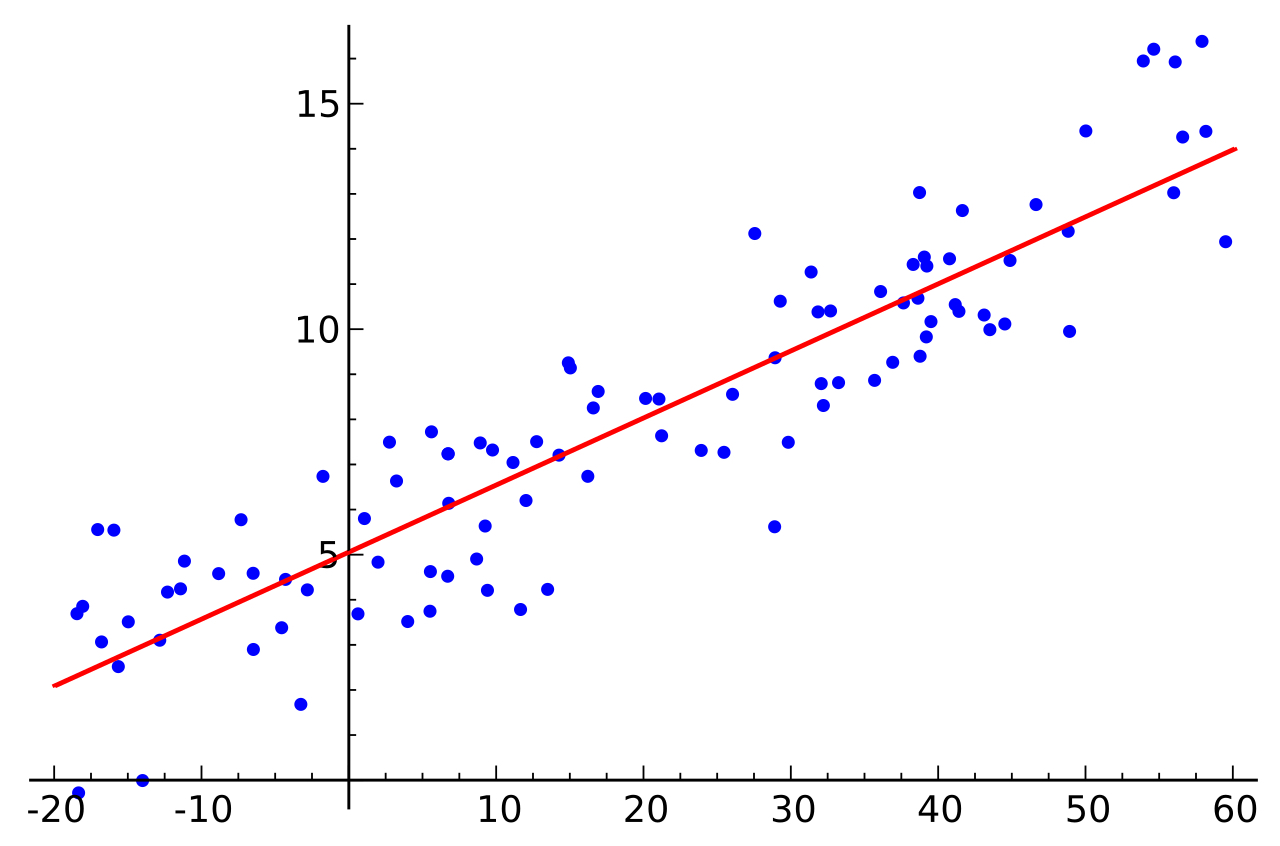
\includegraphics[width=8.5cm, height=3.5cm]{figures/1280px-Linear_regression.jpg}
			\caption{Imagen a la Izquierda}
			\label{Fig:ImagenALaIzquierda}
\end{wrapfigure}

Texto Texto Texto Texto Texto Texto Texto Texto Texto Texto Texto Texto Texto Texto Texto Texto Texto Texto Texto Texto
Texto Texto Texto Texto Texto Texto Texto Texto Texto Texto Texto Texto Texto Texto Texto Texto Texto Texto Texto Texto
Texto Texto Texto Texto Texto Texto Texto Texto Texto Texto Texto Texto Texto Texto

\begin{wrapfigure}[11]{r}[1pt]{8.5cm}
	    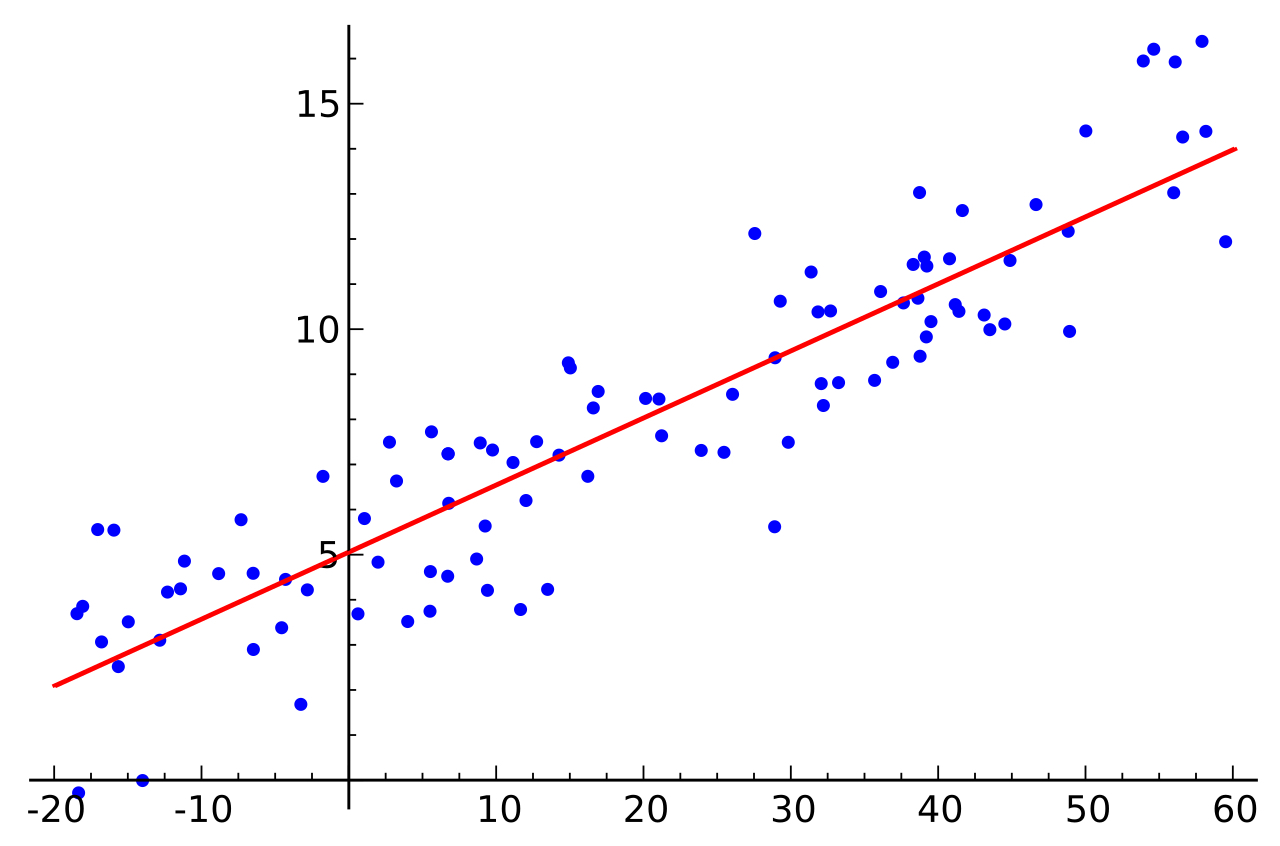
\includegraphics[width=8.5cm, height=3.5cm]{figures/1280px-Linear_regression.jpg}
			\caption{Imagen a la Derecha}
			\label{Fig:ImagenALaDerecha}
\end{wrapfigure}

Texto Texto Texto Texto Texto Texto Texto Texto Texto Texto Texto Texto Texto Texto Texto Texto Texto Texto Texto Texto
Texto Texto Texto Texto Texto Texto Texto Texto Texto Texto Texto Texto Texto Texto Texto Texto Texto Texto Texto Texto
Texto Texto Texto Texto Texto Texto Texto Texto Texto Texto Texto Texto Texto Texto 

\begin{figure}[ht]
	\centering
		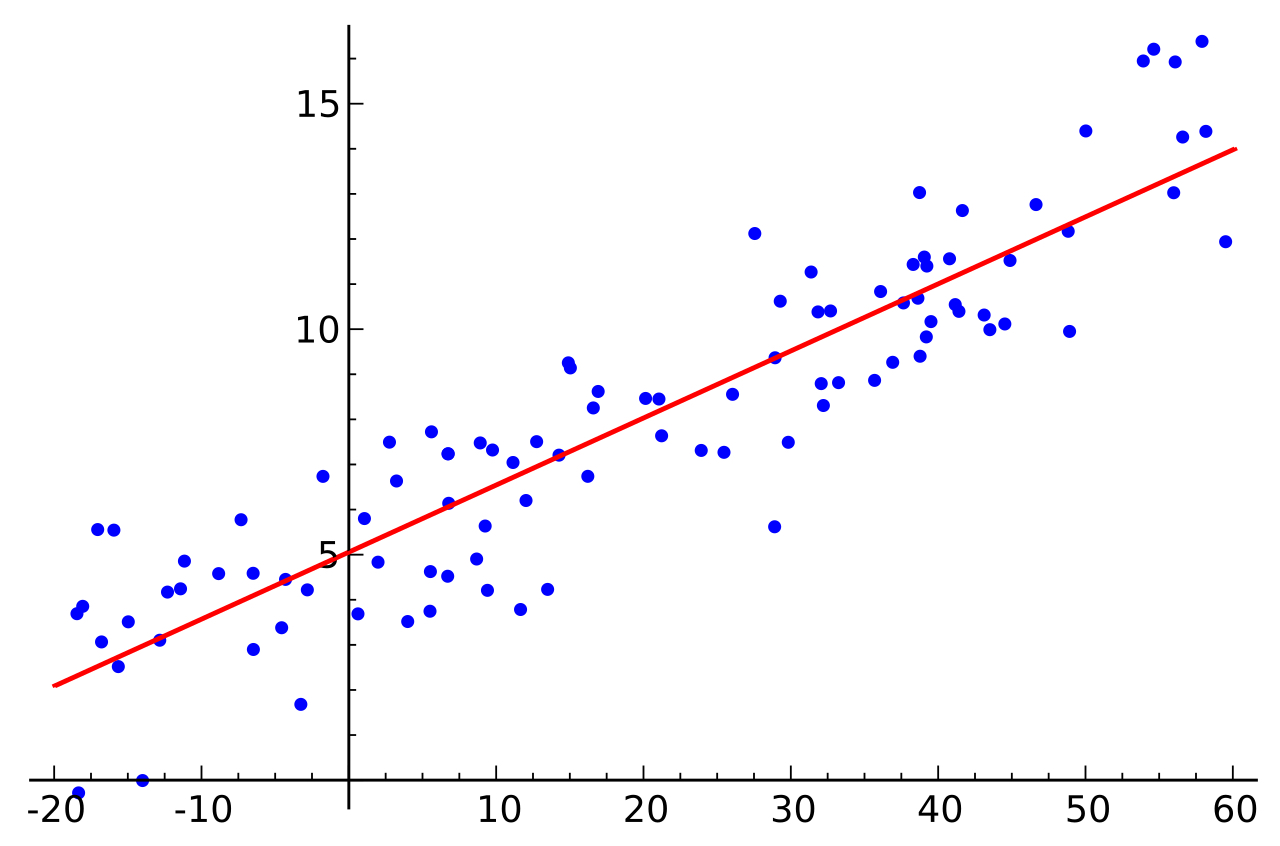
\includegraphics[width=5.5cm]{figures/1280px-Linear_regression.jpg}
	\caption{Imagen Centrada sin Texto}
	\label{Fig:CentradaSinTexto}
\end{figure}

\begin{figure}
   \begin{minipage}{.5\linewidth}
	    \centering
      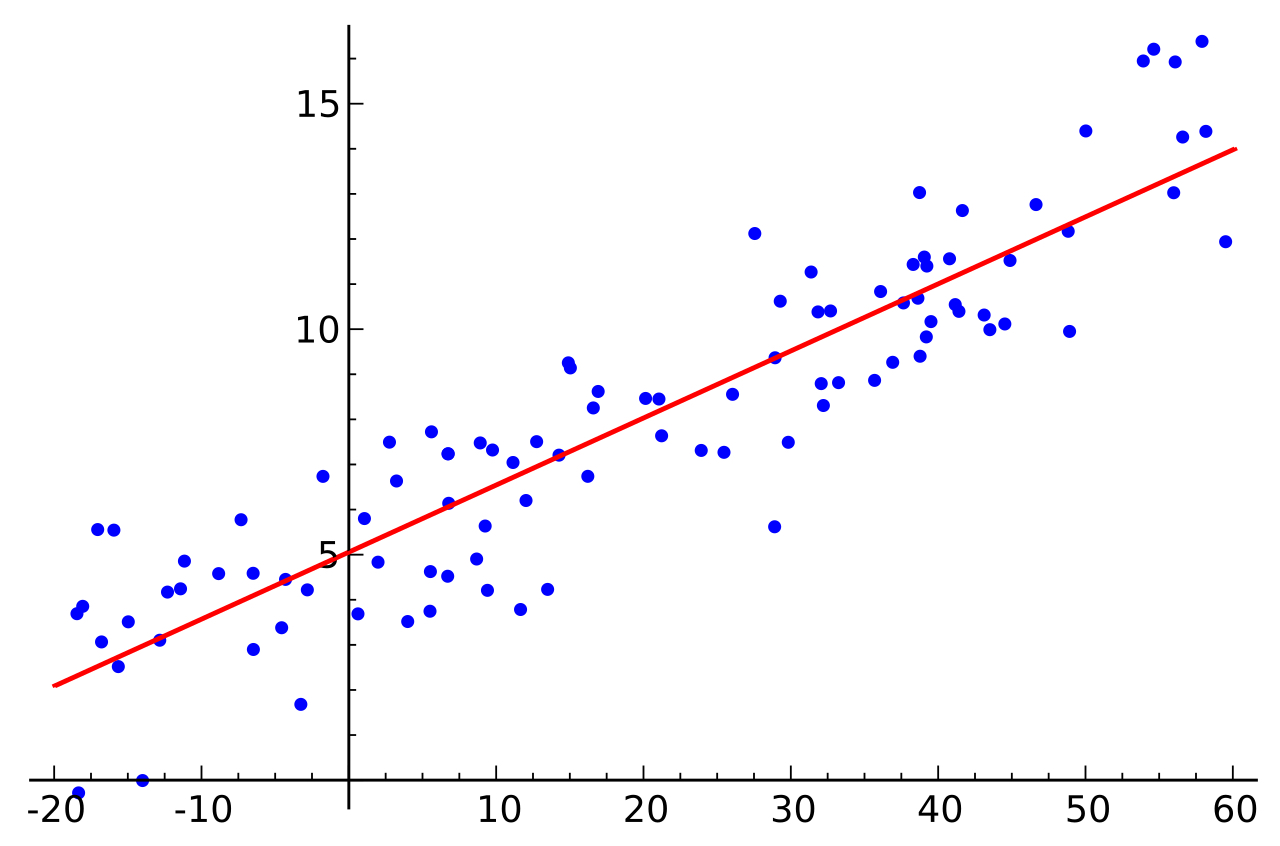
\includegraphics[width=7cm]{figures/1280px-Linear_regression.jpg}
      \caption{Imagen 1}
	 	  \label{Fig:Dos1}
   \end{minipage}%
   \begin{minipage}{.5\linewidth}
	    \centering
		  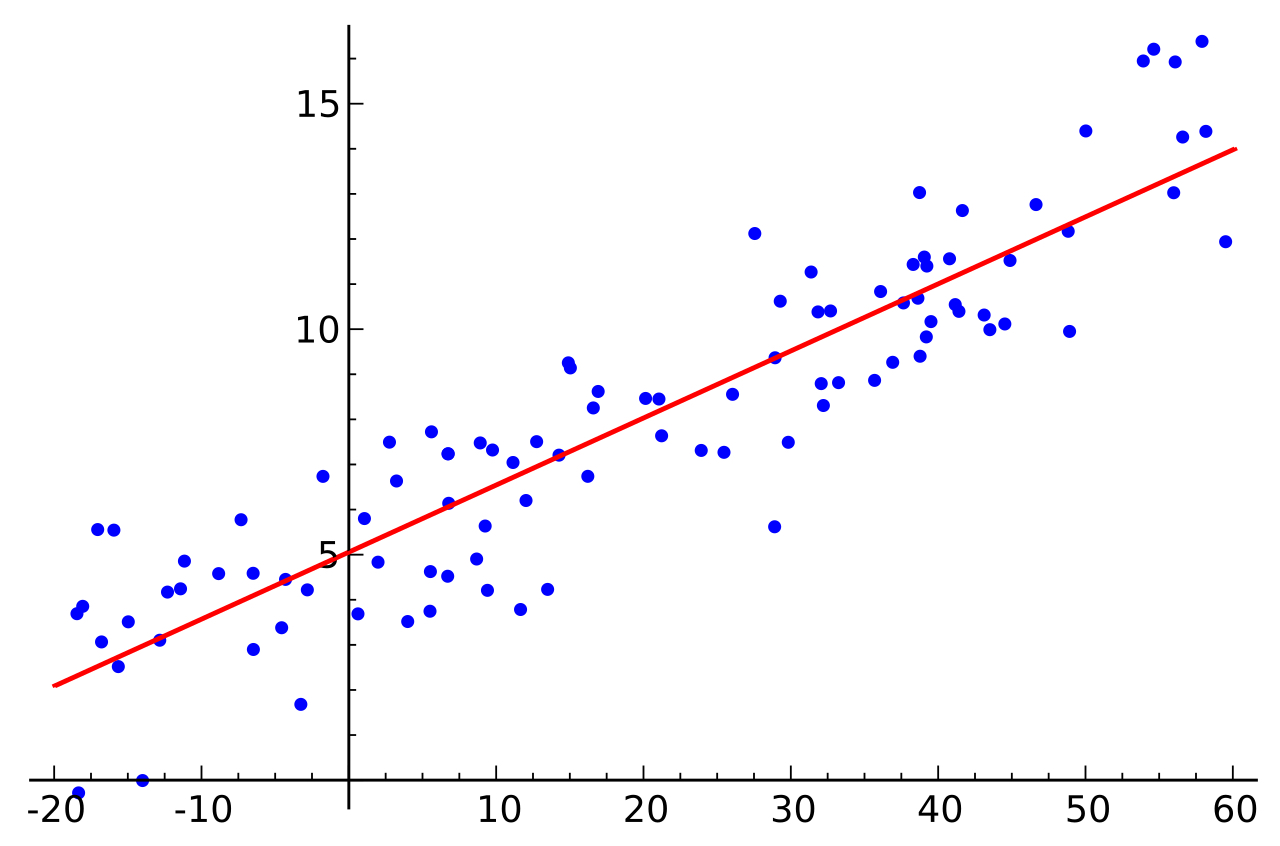
\includegraphics[width=4cm]{figures/1280px-Linear_regression.jpg}
      \caption{Imagen 2}
			\label{Fig:Dos2}
   \end{minipage}
\end{figure}

\newpage
\section{Apéndice B- Referencias Bibliográficas}
\label{Apx:Apendice_B}
%\include{Incluir Fichero Apéndice B}

Estas son algunas referencias bibliográficas, extraidas de \textbf{CiteSeer}:

Algunos libros que hacen referencia a Latex los encontramos en \cite{kreher05pseudocode}, \cite{ohl97emp}, \cite{smith-tools}, \cite{souza-mathematical}, \cite{braams-babel}, \cite{-basic}

\newpage
\bibliographystyle{plain}
\bibliography{Bibliografia}

\end{document}
